% Chapter Template
\chapter{Introduction} % Main chapter title

\label{Chapter1} % Change X to a consecutive number; for referencing this chapter elsewhere, use \ref{ChapterX}

\lhead{Section 1. \emph{Introduction}} % Change X to a consecutive number; this is for the header on each page - perhaps a shortened title

%----------------------------------------------------------------------------------------
%	SECTION 1
%----------------------------------------------------------------------------------------

\section{Introduction to Wavelet Transform}

Generally speaking, a wave is defined to be an oscillating function of time or space, for example, sinusoid and cosinousoid are typical waves used in many fields such as Fourier analysis, which expands signals in terms of sinusiods. In reality, fourier transform has proven to be extremely useful in mathematics, science and engineering especially in dealing with periodic signals. A wavelet is a ``small wave'' with its energy concentrated at a small area and is examined to be more efficient in the analysis of nonstationary phenomena. Figure 1.1 and Figure 1.2 illustrate the main difference between a wave and a wavelet, where a wavelet has its finite energy concentrated around a point compared to wave.
% 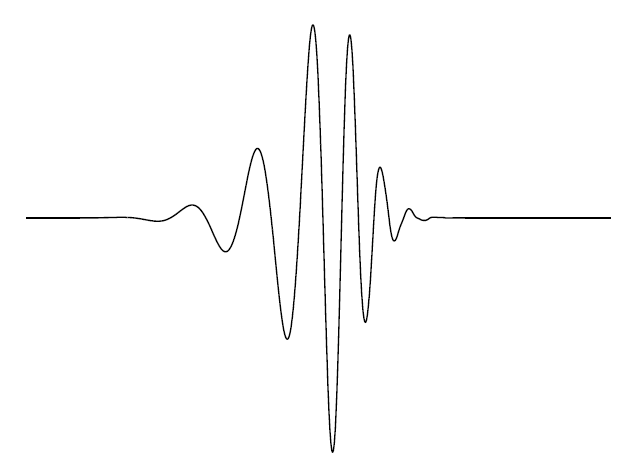
\includegraphics{wavelet.png}
 \begin{figure}[htb]
  \centering
  \begin{minipage}[c]{0.5\textwidth}
\centering
  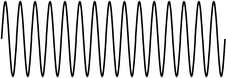
\includegraphics[width=1\linewidth]{sine-wave.png}
  \caption{A Sine Wave}
\end{minipage}%
%注意这个”%”绝对不能省,可以试试不打%的效果
\begin{minipage}[c]{0.5\textwidth}
\centering
  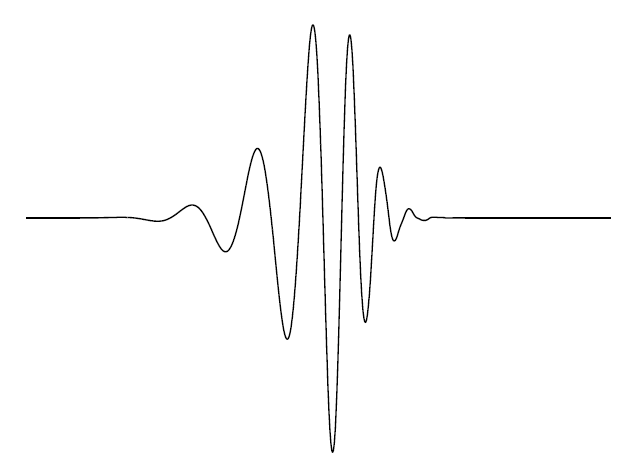
\includegraphics[width=0.6\linewidth]{wavelet.png}
  \caption{Daubechies' Wavelet $\psi_{D20}$}
  \end{minipage}

\end{figure}


%-----------------------------------
%	SUBSECTION 2
%-----------------------------------
\subsection{The Scaling Function}
Scaling functions are defined in order to implement the idea of multiresolution and wavelets are defined in terms of the scaling functions. Moreover, a two-dimensional family of scaling functions are transformed from basic scaling function through translation and scaling by
\begin{equation} \varphi_{j,k}(t) = 2^{j/2}\varphi(2^jt-k) \qquad  k \in \mathbb{Z} \qquad \varphi\in L^2  \end{equation}
and the subspace of $L^2(\mathbb{R})$ spanned by these functions is
\begin{equation} \mathcal{V}_j = \overline{Span_k\{\varphi_{j,k}(t) \}}  \end{equation}
In addition, scaling functions with a lower scale level can be expressed in terms of those at a higher scale by
\begin{equation} \varphi(t) = \sum_n h_0(n)\sqrt2\varphi(2t-n) \end{equation}

%-----------------------------------
%	SUBSECTION 2
%-----------------------------------

\subsection{The Wavelet Functions}
Instead of using $\varphi_{j,k}(t)$ and incresing $j$ to increase the size of the subspace spanned by those scaling functions, a slightly different set of functions $\psi_{j,k}(t)$ which span the differences between the spaces spanned by the various scales of the scaling function is defined by
\begin{equation} \psi(t) = \sum_n h_1(n)\sqrt{2}\varphi(2t-n) \qquad \end{equation}
A signal can be better described by the combination of scaling functions and wavelet functions, especially when the scaling functions and wavelets are orthogonal. Therefore, any function $f(t) \in L^2(\mathbb{R})$ can be represented as 
\begin{equation} f(t) = \sum_{k} c_{j_0}(k)\varphi_{j_0,k}(t) + \sum_k\sum_{j=j_0}^{\infty} d_j(k)\psi_{j,k}(t) \end{equation}


%----------------------------------------------------------------------------------------
%	SECTION 2
%----------------------------------------------------------------------------------------

\section{Introduction to Filter Banks and Discrete Wavelet Transform}
The coefficients $h_0(n)$ and $h_1(n)$ in the equations (1.3) and (1.4) can be viewed as digital filters and the coefficients $c_{j_0}(k)$ and $d_j(k)$ in equations (1.5) can be viewed as digital signals. In signal processing, filter banks contain analysis bank and synthesis bank. Orthogonal wavelet filter banks and tight framelet filter banks will be introduced in the next section and the efficiency of different filter banks will be studied through various experiments.
%-----------------------------------
%	SUBSECTION 2.1
%-----------------------------------

\subsection{Analysis - From Fine Scale to Coarse Scale}
In the process of Decomposition, analysis bank separates the input signal into multiple components with each one carrying different frequency sub-band of the original signal. These multiple components (a collection of sub-signals) can be used to emphasize aspects of the original signal and may help us work with the original signal in an easier and more efficient way. For instance, analysis banks are widely used in signal compression since most useless information can be easily discarded.
Given that $\varphi_{j,k}(t)$ and $\psi_{j,k}(t)$ are orthonormal, the $j^{th}$ level of scaling coefficients are derived from 
\begin{equation} c_j(k) = \langle f(t),\varphi_{j,k}(t)\rangle = \int f(t)2^{j/2}\varphi(2^jt-k)dt \end{equation}
Substituting $\varphi_{j,k}(t)$ with equation (1.1) giving the scaling coefficients
\begin{equation} c_j(k) = \sum_m h_0(m-2k)c_{j+1}(m) \end{equation}
The corresponding formula for the wavelet coefficients can be derived in the same way
\begin{equation} d_j(k) = \sum_m h_1(m-2k)c_{j+1}(m)\end{equation}

%-----------------------------------
%	SUBSECTION 2.2
%-----------------------------------
\subsection{Synthesis - From Coarse Scale to Fine Scale}
 The output of analysis can be reconstructed in the process of Reconstruction with the synthesis bank. Moreover, the desire for perfect reconstruction (i.e., the output signal is exactly the same as the input signal) imposes extra constraints on the analysis and synthesis filters.
 \begin{equation} c_{j+1}(k) = \sum_mc_j(m)h_0(k-2m) + \sum_md_j(m)h_1(k-2m) \end{equation}


%-----------------------------------
%	SUBSECTION 2.3
%-----------------------------------
 \subsection{Discrete Wavelet Transform}
 The classical discrete wavelet transform (DWT) provides means of implementing analysis on the basis of filter banks with the attribute of perfect reconstruction. It has proven to be practically efficient in the process of a certain classes of signals, especially for piecewise smooth signals which will be presented in the following sections. 



